\documentclass[12pt]{article}

\usepackage{sbc-template}
\usepackage{graphicx,url}
\usepackage[utf8]{inputenc}
\usepackage[T1]{fontenc}
\usepackage[brazil]{babel}
\usepackage{booktabs}
\usepackage{tikz}
\usetikzlibrary{arrows.meta,positioning,fit}
\usepackage{caption}

\sloppy
\providecommand{\normalsfcodes}{}

\title{Detecção de Imagens Sintéticas após Transformações Digitais:\\
implementação do detector VerifAI e avaliação}

\author{Nathália G. Ribas\inst{1}, Igor M. da Rosa\inst{1}}

\address{Departamento de Computação (DEC)\\
Universidade Federal de Santa Catarina\\
Araranguá, SC
\email{ribas.nathalia@grad.ufsc.br, igor.matos.rosa@grad.ufsc.br}
}

\begin{document}

\maketitle

\begin{abstract}
This paper continues the previous report on classical detection of AI-generated images under digital transforms. After CIFAKE experiments, we moved to a paired COCO and synthetic dataset built locally with ControlNet Depth, trained FFT, HOG and LBP features with an RBF SVM, and delivered the VerifAI Streamlit app. On a 4{,}000/1{,}000 pair holdout, fusion reaches 88.15\% accuracy and stays robust under light JPEG, resize and blur. We also discuss limits outside the training domain and outline next steps.
\end{abstract}

\begin{resumo}
Este artigo complementa o relatório anterior sobre detecção clássica de imagens geradas por IA sob transformações digitais. Depois dos experimentos no CIFAKE, passamos a uma base pareada COCO e sintética gerada localmente com ControlNet Depth, treinamos FFT, HOG e LBP com SVM RBF e entregamos o aplicativo Streamlit VerifAI. No holdout 4{.}000/1{.}000 pares, a fusão chega a 88,15\% de acurácia e permanece robusta a JPEG, resize e blur leves. Também discutimos os limites fora do domínio treinado e os próximos passos.
\end{resumo}

%----------------------------------------------------------------------
\section{Introdução}
%----------------------------------------------------------------------

Imagens geradas por inteligência artificial circulam com facilidade em redes sociais, campanhas e anúncios. Na prática, quase nunca chegam intactas: passam por compressão JPEG, recorte, redimensionamento e filtros. Um detector pode acertar a foto limpa e errar depois dessas mudanças. Esse comportamento aparece em ferramentas públicas, como o ZeroGPT\footnote{\url{https://www.zerogpt.com/pt/ai-image-detector}} (Figura~\ref{fig:zerogpt}): a mesma cena marcada como falsa passa a ser tratada como real após uma compressão simples.

\begin{figure}[ht]
\centering
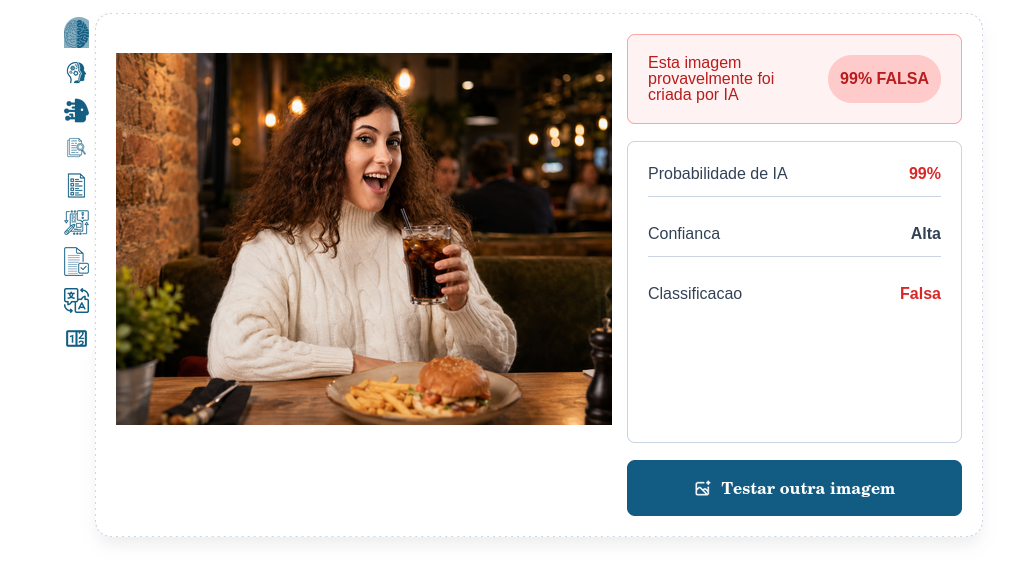
\includegraphics[width=0.48\textwidth]{suporte/TestePosTransformacao.png}
\hfill
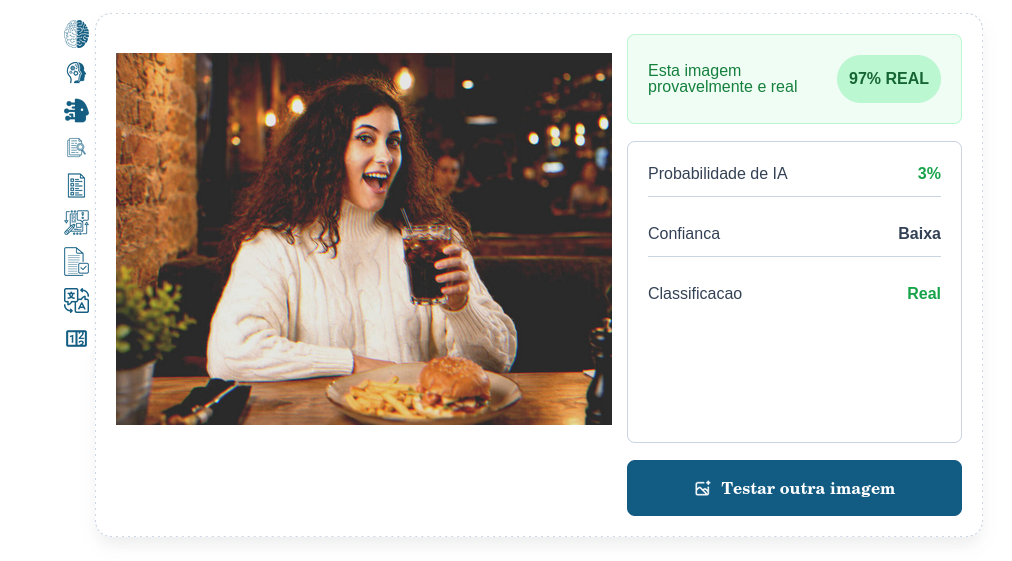
\includegraphics[width=0.48\textwidth]{suporte/TesteReducaoReso.png}
\caption{Teste com ZeroGPT. À esquerda, cena alterada por IA marcada como falsa. À direita, a mesma imagem após compressão passa a ser tratada como real.}
\label{fig:zerogpt}
\end{figure}

A pergunta que guia o projeto é: quão bem detectores baseados em features clássicas continuam funcionando quando a imagem sofre transformações típicas da internet? No relatório anterior, essa pergunta foi respondida no CIFAKE~\cite{bird2024cifake}, com descritores FFT, HOG e LBP e um SVM de kernel RBF~\cite{cortes1995svm,dalal2005hog,ojala2002lbp,gonzalez2018}. Treinar só nas imagens originais deu cerca de 92\% de acurácia no teste limpo, mas a fusão caiu para perto de 54\% após crop, blur ou o pipeline combinado. Incluir as transformações no treino recuperou a robustez (fusão acima de 71\% no mesmo pipeline), ao custo de uma queda moderada no teste original.

Ainda assim, o CIFAKE em $32{\times}32$ e no domínio do CIFAR-10 ficou longe do uso em fotos reais de celular. Surgiram duas questões práticas para a continuação do trabalho. A primeira é escolher uma base adequada para um aplicativo de inspeção. A segunda é alinhar REAL e FAKE: sem o par inverso (mesma cena e mesma pose), o classificador tende a aprender o assunto da foto, e não o sinal de que a imagem foi gerada.

Este artigo descreve essa etapa final. Na Seção~\ref{sec:desenvolvimento} apresentamos as escolhas de desenvolvimento e a implementação do detector VerifAI (features, parâmetros, letterbox e aplicativo Streamlit). Na Seção~\ref{sec:avaliacao} detalhamos a metodologia de avaliação e os resultados na base pareada. Na Seção~\ref{sec:conclusao} discutimos se o objetivo foi atingido e os trabalhos futuros.

%----------------------------------------------------------------------
\section{Desenvolvimento}
\label{sec:desenvolvimento}
%----------------------------------------------------------------------

A partir da fundamentação e dos experimentos da entrega anterior, o desenvolvimento concentrou-se em três decisões: qual base usar no app, como pré-processar a imagem e quais variantes digitais entram no treino.

\subsection{Escolhas finais de base e alinhamento REAL/FAKE}

O CIFAKE validou o pipeline clássico, porém a resolução baixa e o domínio fechado não transferiram bem para fotos de celular. Tentativas com CelebA só como REAL e com coleções de IA de rede sem REAL proporcional do mesmo tipo de cena também falharam na prática: o classificador aprendia o assunto da foto (rosto de estúdio, estilo de post) em vez do sinal de síntese. No cruzamento COCO (REAL diverso) com FAKE de rede social, a FFT ficou perto do acaso (cerca de 53\%).

A escolha final foi gerar 5{.}000 pares locais: cada foto real do COCO~\cite{coco2017} recebe uma versão sintética com a mesma pose e composição. O fluxo usa BLIP para descrever a cena e Stable Diffusion 1.5 com ControlNet Depth (profundidade MiDaS) para gerar a imagem IA. Assim, REAL e FAKE passam a ser o par inverso, e o SVM aprende a diferença de aparência, e não só o conteúdo.

A Figura~\ref{fig:par} mostra um exemplo de par. A Figura~\ref{fig:fluxo} resume o fluxo final do detector.

\begin{figure}[ht]
\centering
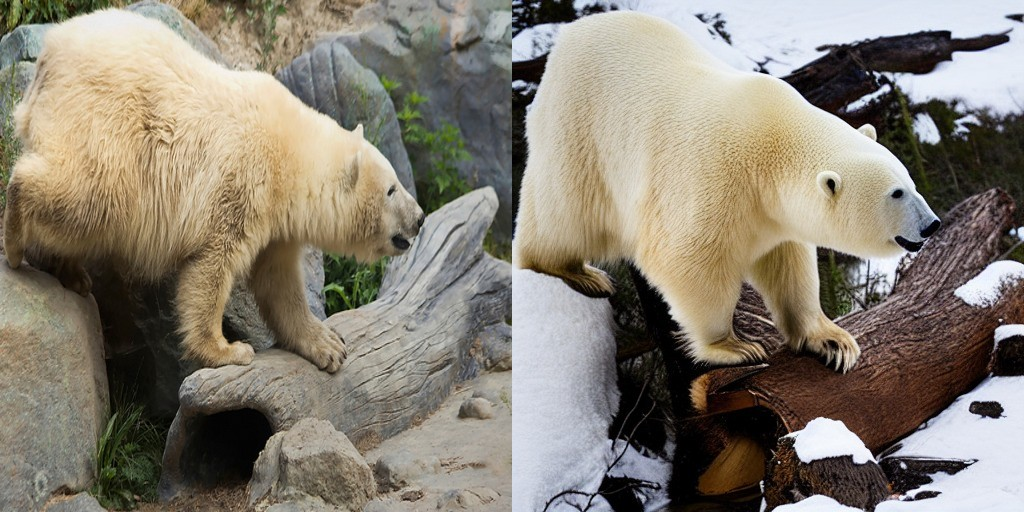
\includegraphics[width=0.95\textwidth]{suporte/par_real_ia.jpg}
\caption{Exemplo de par REAL (esquerda) e IA (direita) usado no treino final.}
\label{fig:par}
\end{figure}

\begin{figure}[ht]
\centering
\begin{tikzpicture}[
  node distance=0.55cm,
  box/.style={draw, rounded corners, align=center, font=\footnotesize,
              inner sep=5pt, minimum width=3.2cm},
  arr/.style={-{Latex}, thick}
]
  \node[box, fill=gray!12] (b) {Base pareada\\COCO e IA};
  \node[box, below=of b] (e) {Letterbox 224\\+ FFT / HOG / LBP};
  \node[box, below=of e] (t) {SVM RBF\\4k/1k pares};
  \node[box, below=of t, fill=green!12] (a) {App VerifAI\\fusão + scores};
  \draw[arr] (b) -- (e);
  \draw[arr] (e) -- (t);
  \draw[arr] (t) -- (a);
\end{tikzpicture}
\caption{Fluxo final: da base pareada ao aplicativo VerifAI.}
\label{fig:fluxo}
\end{figure}

\subsection{Pré-processamento e aumento de dados}

Diferente do CIFAKE ($32{\times}32$), o pipeline final encaixa a foto inteira em $224{\times}224$ mantendo a proporção (letterbox). A borda usa reflexão, e não preenchimento preto, porque faixas pretas criavam anéis artificiais no espectro FFT. O HOG usa resolução interna de $128{\times}128$. Treino e app passam pelo mesmo formato.

No treino entram seis variantes leves da mesma imagem: original, JPEG 90 e 70, resize à metade, blur gaussiano $3{\times}3$ e um pipeline que combina crop de 25\%, resize $0{,}5$ e JPEG 70. Crops fortes e JPEG 50 ficam só na avaliação de robustez. A ideia é preparar o modelo para a circulação digital sem apagar o sinal que a FFT precisa aprender.

\subsection{Implementação}
\label{sec:implementacao}

A implementação mantém a linha clássica escolhida antes: descritores FFT, HOG e LBP concatenados (fusão) e SVM com kernel RBF~\cite{cortes1995svm,dalal2005hog,ojala2002lbp,gonzalez2018}. A Tabela~\ref{tab:dims} resume as dimensões no pipeline final.

\begin{table}[ht]
\centering
\caption{Dimensões dos descritores no detector final.}
\label{tab:dims}
\begin{tabular}{lrl}
\toprule
Descritor & Dimensão & Observação \\
\midrule
FFT   & 68    & 64 anéis + 3 bandas + centróide \\
HOG   & 1{.}568 & resolução interna $128{\times}128$ \\
LBP   & 10    & uniforme $P{=}8$, $R{=}1$ \\
Fusão & 1{.}646 & concatenação padronizada \\
\bottomrule
\end{tabular}
\end{table}

A FFT 2D é aplicada em escala de cinza, com espectro centralizado, magnitude logarítmica e perfil radial. Não há normalização min-max por imagem, para preservar diferenças absolutas de energia de alta frequência. Cada família de features é padronizada com \texttt{StandardScaler} ajustado só no treino. Os parâmetros do SVM são $C{=}10$ e $\gamma{=}\mathrm{auto}$, com peso maior na classe REAL para reduzir falso positivo no aplicativo. O treino usa ThunderSVM na GPU e, se preciso, \texttt{sklearn} na CPU.

O protocolo de avaliação usa 4{.}000 pares no treino (8{.}000 imagens) e 1{.}000 pares no teste (2{.}000 imagens), com divisão por par e semente fixa. Cada imagem de treino gera seis amostras (as variantes acima), cerca de 48{.}000 vetores por família. O aplicativo Streamlit (VerifAI) refaz o mesmo caminho: letterbox 224, extração das features, scalers do treino e probabilidade de conteúdo sintético pela fusão. Entre 40\% e 60\% o resultado é tratado como inconclusivo; scores de FFT e HOG aparecem como apoio.

%----------------------------------------------------------------------
\section{Avaliação}
\label{sec:avaliacao}
%----------------------------------------------------------------------

A avaliação mede a acurácia no holdout de pares e a queda após transformações digitais, sem retreinar o classificador. A base de teste compartilha a distribuição do treino (ambos do universo COCO pareado), o que avalia generalização dentro desse domínio, e não para a web aberta.

\subsection{Metodologia}

Para cada imagem do holdout calculam-se FFT, HOG, LBP e a fusão. Treinam-se quatro SVMs (um por família e um de fusão). No teste limpo reportam-se acurácia, precisão na classe FAKE e recall na classe REAL. Na robustez, as mesmas imagens de teste passam por JPEG 90, 70 e 50, resize $0{,}5$, blur $3{\times}3$, crops de 10\%, 25\% e 40\% e o pipeline combinado. A métrica principal continua sendo a acurácia da fusão, o detector usado no app.

\subsection{Resultados no holdout}

A Tabela~\ref{tab:v3} resume o teste limpo. A fusão chega a 88,15\%. HOG (84,40\%) e LBP (82,30\%) ficam acima da FFT isolada (75,00\%) neste domínio. A concatenação dá o melhor equilíbrio entre precisão em FAKE e recall em REAL.

\begin{table}[ht]
\centering
\caption{Acurácia no holdout de pares (4{.}000 treino / 1{.}000 teste). SVM RBF.}
\label{tab:v3}
\begin{tabular}{lrrr}
\toprule
Feature & Acurácia & Prec.\ FAKE & Rec.\ REAL \\
\midrule
FFT    & 0,7500 & 0,799 & 0,832 \\
HOG    & 0,8440 & 0,887 & 0,899 \\
LBP    & 0,8230 & 0,860 & 0,874 \\
\textbf{Fusão} & \textbf{0,8815} & 0,865 & 0,859 \\
\bottomrule
\end{tabular}
\end{table}

\subsection{Robustez às transformações}

A Figura~\ref{fig:rob} e a Tabela~\ref{tab:rob} mostram a acurácia por transformação. JPEG leve, resize e blur mantêm a fusão em geral acima de 87\%. Crops fortes e o pipeline provocam a maior queda: 74,50\% no crop de 40\% e 79,55\% no pipeline, ainda acima do acaso. O mapa da Figura~\ref{fig:heat} indica que a FFT sofre mais com crop e compressão forte, enquanto HOG e a fusão absorvem melhor parte dessas mudanças.

\begin{figure}[ht]
\centering
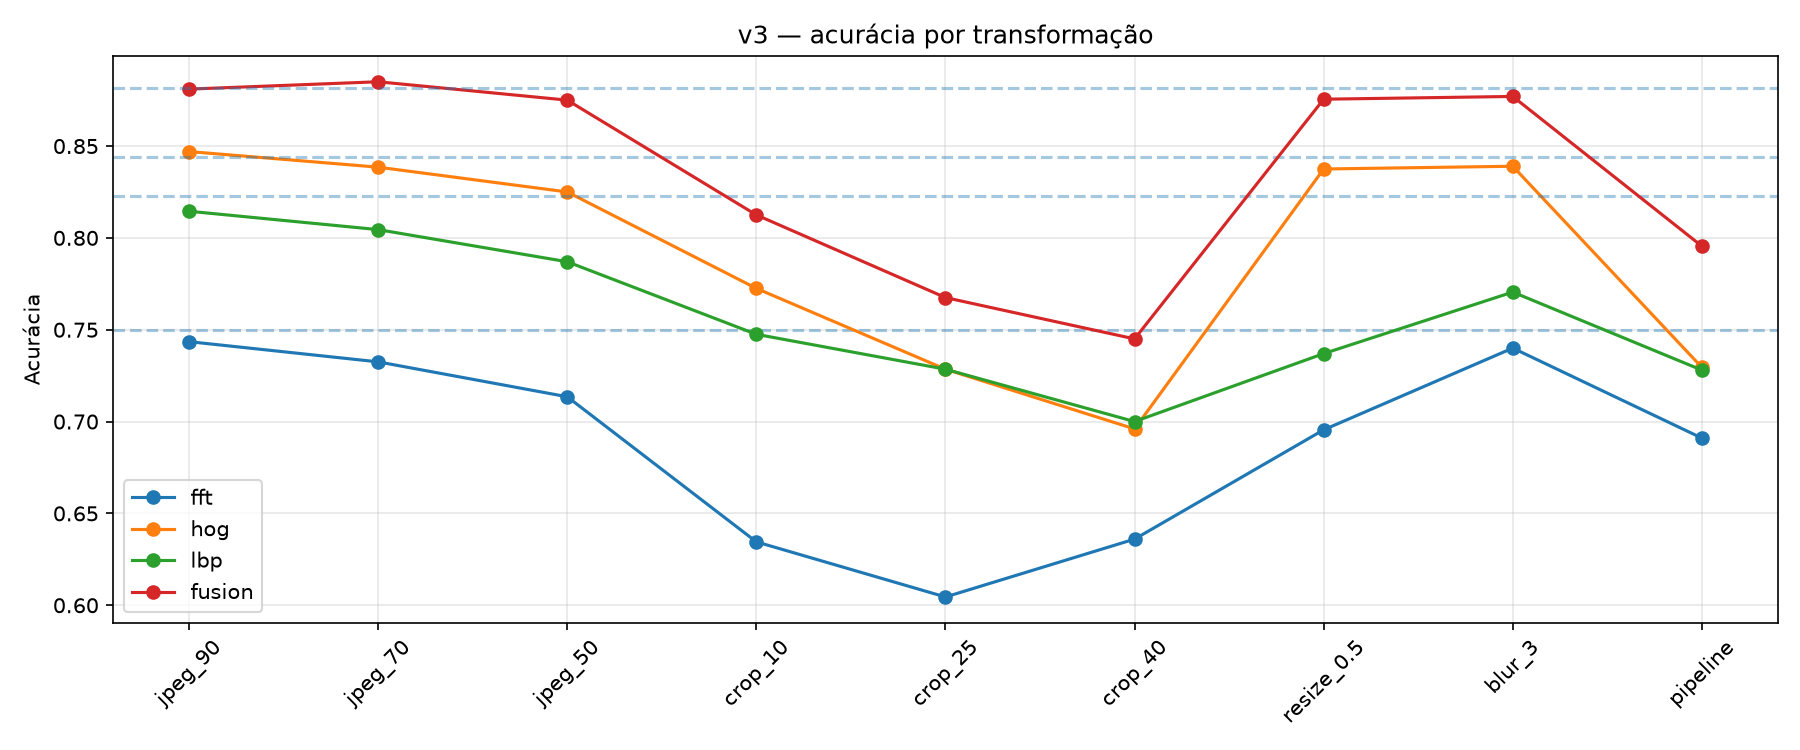
\includegraphics[width=\textwidth]{suporte/v3_acc_por_transf.png}
\caption{Acurácia por transformação no holdout (pares).}
\label{fig:rob}
\end{figure}

\begin{table}[ht]
\centering
\small
\caption{Acurácia da fusão por transformação no holdout (baseline 0,8815).}
\label{tab:rob}
\begin{tabular}{lrr}
\toprule
Transformação & Acurácia fusão & Queda \\
\midrule
JPEG 90      & 0,8810 & 0,0005 \\
JPEG 70      & 0,8850 & $-$0,0035 \\
JPEG 50      & 0,8750 & 0,0065 \\
Resize $0{,}5$ & 0,8755 & 0,0060 \\
Blur $3{\times}3$ & 0,8770 & 0,0045 \\
Crop 10\%    & 0,8125 & 0,0690 \\
Crop 25\%    & 0,7675 & 0,1140 \\
Crop 40\%    & 0,7450 & 0,1365 \\
Pipeline     & 0,7955 & 0,0860 \\
\bottomrule
\end{tabular}
\end{table}

\begin{figure}[ht]
\centering
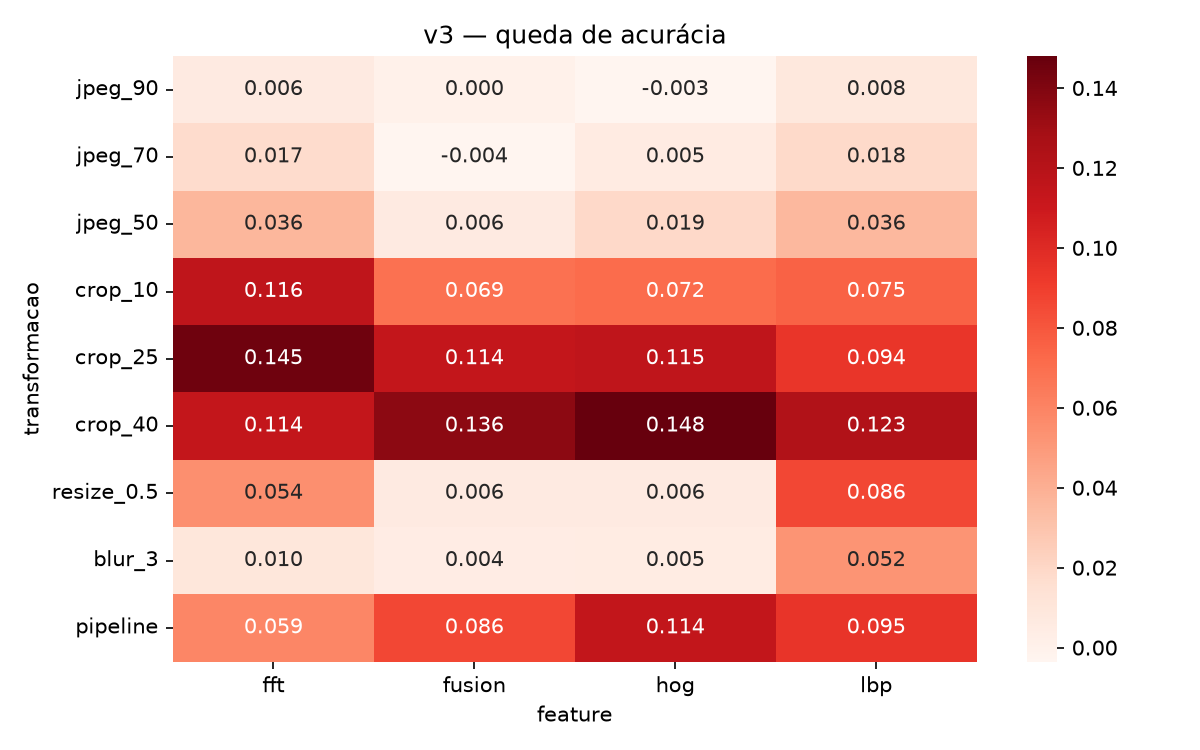
\includegraphics[width=0.92\textwidth]{suporte/v3_heatmap_queda.png}
\caption{Mapa de queda de acurácia por feature e transformação.}
\label{fig:heat}
\end{figure}

Comparando com o CIFAKE da entrega anterior (cerca de 92\% no original e queda forte após crop ou blur sem aumento adequado) e com o cruzamento Harvard e COCO (cerca de 53\% na FFT), a base pareada recupera precisão e se aproxima melhor do uso do app, desde que a imagem de teste esteja ligada ao universo treinado.

As Figuras~\ref{fig:ex-real} e~\ref{fig:ex-ia} ilustram saídas típicas do VerifAI em inspeção manual.

\begin{figure}[ht]
\centering
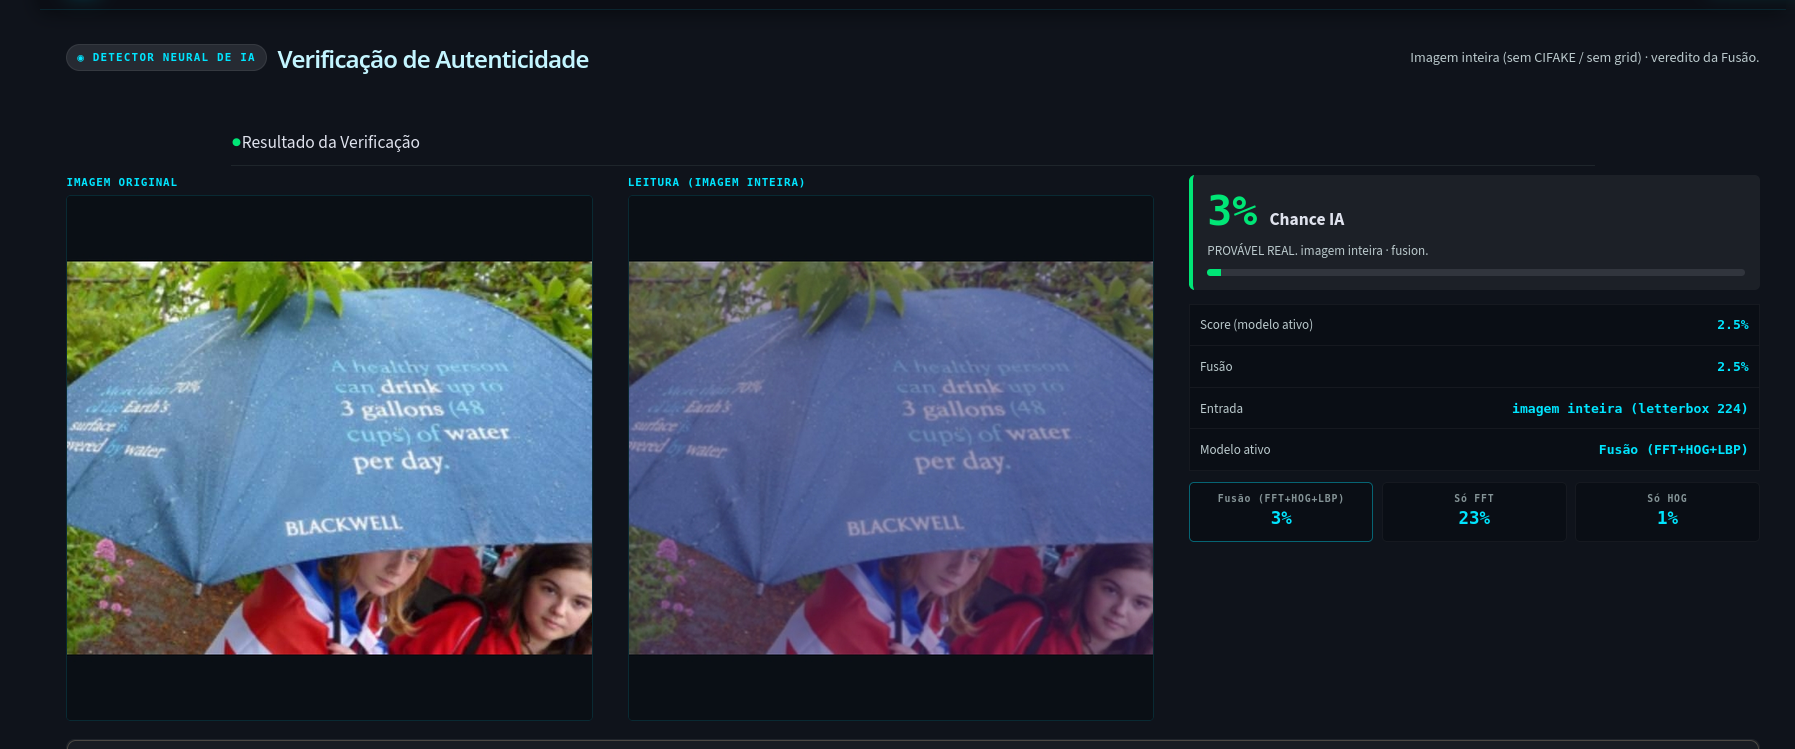
\includegraphics[width=\textwidth]{suporte/ExReal.png}
\caption{Exemplo no app: foto real classificada como provável real.}
\label{fig:ex-real}
\end{figure}

\begin{figure}[ht]
\centering
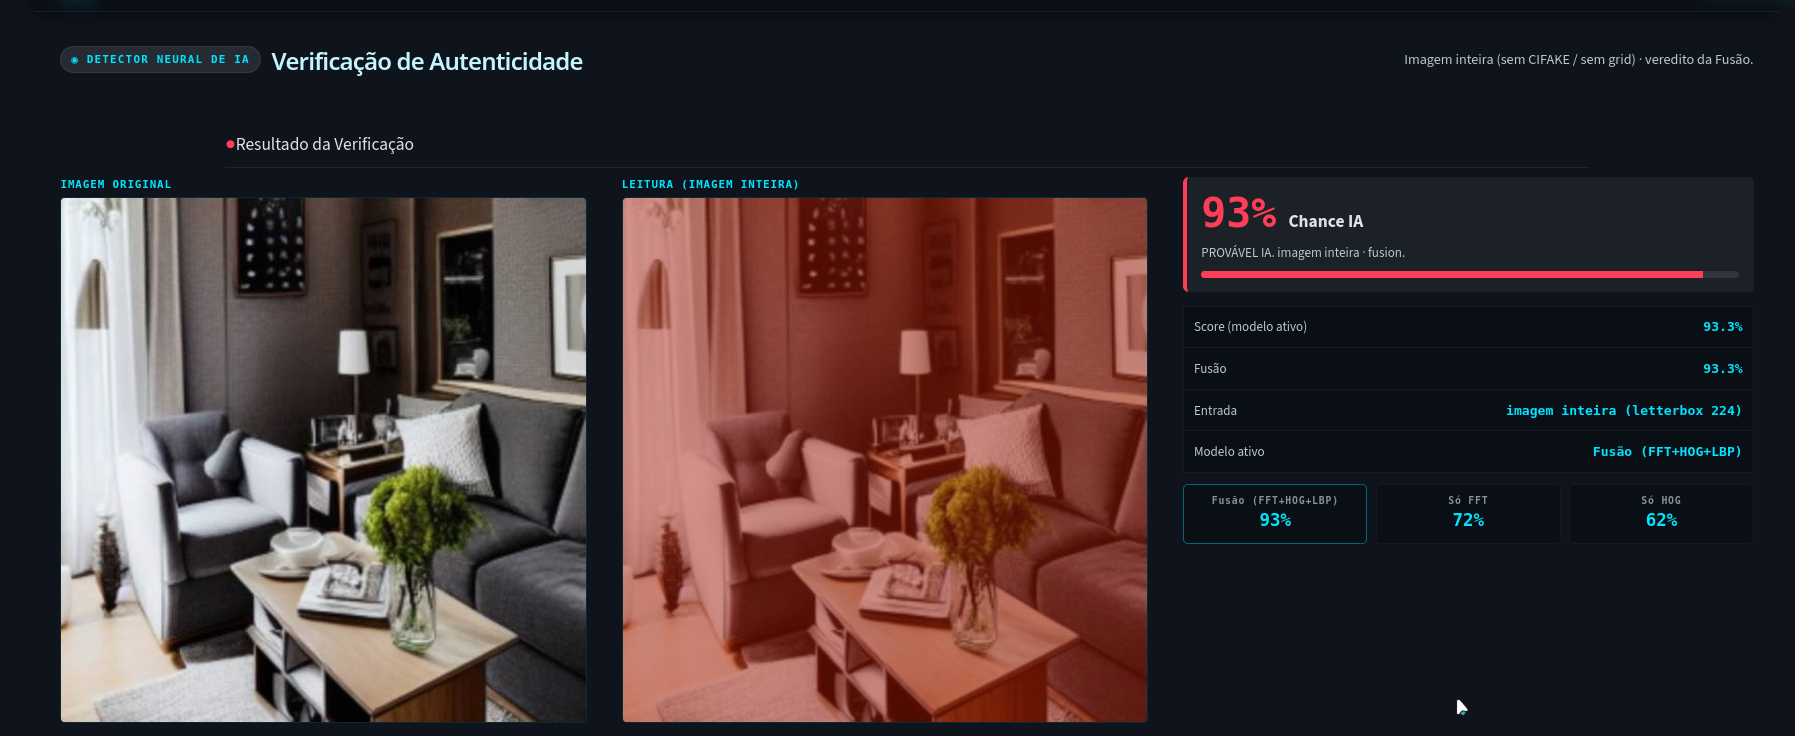
\includegraphics[width=\textwidth]{suporte/ExIA.png}
\caption{Exemplo no app: imagem sintética classificada como provável IA.}
\label{fig:ex-ia}
\end{figure}

\subsection{Discussão dos resultados}

Os pares com ControlNet ensinam a diferença entre a mesma cena real e a mesma cena sintética. A fusão (88,15\%) fica acima da FFT isolada (75\%), o que sugere que HOG e LBP complementam o espectro quando a geometria é compartilhada. Dentro do domínio e sob as transformações do escopo inicial, o detector cumpre o objetivo de robustez no app.

Fora desse domínio, com imagens bem diferentes das treinadas (outros geradores, selfies fortes, prints de tela), o SVM com features manuais perde precisão e confunde REAL com IA. Isso é esperado: os descritores são fixos e não criam representações novas quando o estilo visual muda. Para um detector mais geral, deep learning seria o próximo passo natural~\cite{bird2024cifake}. Para este trabalho, com foco em interpretar o modelo e entregar um app clássico, o SVM permanece adequado.

%----------------------------------------------------------------------
\section{Conclusão}
\label{sec:conclusao}
%----------------------------------------------------------------------

O objetivo do projeto era medir a robustez de um detector clássico após transformações digitais e entregar uma solução utilizável. Esse objetivo foi atingido no domínio da base pareada: a fusão chegou a 88,15\% no holdout 4{.}000/1{.}000 e se manteve acima de 87\% em JPEG, resize e blur leves, com o VerifAI avaliando a imagem inteira no mesmo formato do treino.

A principal lição de desenvolvimento é que a base importa tanto quanto o classificador. CIFAKE, CelebA e FAKE de rede sem REAL inverso não bastaram para o app. Só com pares COCO e IA alinhados em cena e pose o SVM passou a separar síntese de conteúdo.

Como trabalhos futuros, duas linhas se destacam. A primeira é especializar a detecção em duas etapas: identificar o tipo de transformação e depois aplicar um modelo REAL/IA treinado para aquele caso. A segunda é reforçar a base com dados mais próximos do que circula na internet, mantendo REAL e FAKE proporcionais do mesmo contexto. Com volume e diversidade suficientes, a migração de SVM com features manuais para deep learning também passa a fazer sentido.

\bibliographystyle{sbc}
\bibliography{referencias}

\end{document}
